\documentclass{article}

\usepackage[margin=20pt]{geometry}
\usepackage{graphicx}
\graphicspath{{figures/}{../figures/}}

\usepackage{tikz}
\usetikzlibrary{3d, calc, external}
\tikzexternalize[prefix=figures-cache/]

\usepackage{amsmath, amssymb, amsfonts}

\newcommand{\ie}{{\it i.e.~}}
\newcommand{\eg}{{\it e.g.~}}
\newcommand{\nb}{{\it n.b.~}}
\newcommand{\cfr}{{\it cfr.~}}
\newcommand{\viz}{{\it viz.~}}
\newcommand{\etc}{{\it etc.~}}
\newcommand{\sic}{{\it sic.~}}
\newcommand{\wrt}{{w.r.t.~}}

\usepackage{pgfplots}
\pgfplotsset{compat=1.18}

\usepackage{quantikz}
\usepackage{braket}
\usepackage{subcaption}
\usepackage{hyperref}

\colorlet{quantumR}{red!75!black!50}
\colorlet{quantumB}{blue!75!black!50}
\colorlet{quantumG}{green!75!black!50}
\colorlet{quantumY}{yellow!95!black!75}
\colorlet{quantumP}{magenta!75}

\tikzstyle{data}=[circle, fill=black, text=white]
\tikzstyle{meas}=[circle, fill=white, draw=black, ultra thick]
\tikzstyle{stabilizer}=[draw=black]

\tikzset{
  bfg/.style={rounded corners=5pt, minimum height=5.5cm}
}
\tikzset{
  bfgps/.style={rounded corners=5pt, minimum height=5.5cm, fill=gray}
}

\newcommand{\ttbf}{\ttfamily\fontseries{b}\selectfont}
\DeclareMathAlphabet{\mathpzc}{OT1}{pzc}{m}{it}

\newcommand{\parentheses}[1]{\left(\vphantom{\sum}#1\right)}
\newcommand{\brackets}[1]{\left[\vphantom{\sum}#1\right]}
\newcommand{\Sup}[1]{^{\scriptscriptstyle #1}}
\newcommand{\sub}[1]{_{\scriptscriptstyle #1}}

\newcommand{\qmeasure}[1]{\meter{\raisebox{-24pt}[\height][0pt]{\scalebox{0.5}{#1}}}}

\title{TQEC --- Notes on Magic State Cultivation\thanks{Based on Austin Fowler's presentations of \texorpdfstring{\href{https://arxiv.org/abs/arXiv:2510.24615}{arXiv:2510.24615}}{arXiv:2510.24615} and \texorpdfstring{\href{https://arxiv.org/abs/2510.24615}{arXiv:2409.17595}}{arXiv:2409.17595} at TQEC meetings on 2026/08/12 and 2026/08/19}}
\author{Seweryn Dynerowicz}
%\date{}

\newcommand{\Op}[1]{{\bf #1}}
\newcommand{\kett}[1]{\ket{\mbox{\tt #1}}}
\newcommand{\swt}[1]{\setwiretype{#1}}

\begin{document}
	\maketitle

	\section{Stage I --- Preparation}
	
	The goal of this stage is to prepare a logical magic state\footnote{We'll use this term to refer to either logical states; $\ket{\Op{S}}\sub{L}$ or $\ket{\Op{T}}\sub{L}$} encoded\footnote{Note that the $\kett{0}\sub{L}$ and $\kett{1}\sub{L}$ are the logical states of the Steane Code, not the physical ones} with the Steane Code on $7$ data-qubits (code distance $3$). Since performing simulations and computations with $\Op{T}$ gates incurs an exponential penalty in the classical setting, Gidney uses $\Op{S}$ gates as {\it proxies} and operates under an assumption that the logical error rates between the two scenarios are related by a factor of $2$.
	\begin{equation}
		\ket{\Op{S}}\sub{L} ~=~
			\sqrt{\frac{1}{2}}\left(\vphantom{\sqrt{\frac{1}{2}}}
				\kett{0}\sub{L} + e^{i\pi/2}\kett{1}\sub{L}
			\right)
		\qquad\qquad\qquad
		\ket{\Op{T}}\sub{L} ~=~
			\sqrt{\frac{1}{2}}\left(\vphantom{\sqrt{\frac{1}{2}}}
				\kett{0}\sub{L} + e^{i\pi/4}\kett{1}\sub{L}
			\right)
		\label{eq:magic-states}
	\end{equation}

	The preparation stage is broken down into three main parts as shown in the figure below. In the \textsc{Injection} part, an attempt is made to prepare a logical magic state using a modified Steane Code circuit where a phase of $e^{i\pi/2}$ (resp. $e^{i\pi/4}$) is injected into a logical $\kett{+}\sub{L}$ state. \\

	Since we are working in a noisy environment, that attempt may fail and we wish to confirm whether the state that was prepared is indeed the one from Eq. (\ref{eq:magic-states}). This is achieved by post-selecting based on a \textsc{Steane} check and a \textsc{Phase} check. If any measured syndrome in those checks is non-zero, we discard the state and attempt again from the \textsc{Injection}. By allowing multiple attempts to be made, we improve the logical error rate achieved beyond the raw physical error rate. \\
	
	The \textsc{Steane Check} involves measuring the stabilisers of the Steane Code in order to determine whether the state lies in the correct code-space or has been corrupted. The \textsc{Phase Check} involves measuring a \Op{Y} stabiliser (resp. $\Op{H}\sub{XY}$) to confirm that the state has the correct relative phase between the states $\kett{0}\sub{L}$ and $\kett{1}\sub{L}$.

	\begin{figure}[h!]
		\centering
		\begin{quantikz}[row sep={between origins, 0.75cm}]
			& \gate[7, style=bfg][3cm]{\large\textsc{Injection}}
			& \gate[7, style=bfgps][3cm]{\large\shortstack{\color{white}\sc Steane \\ \color{white}\sc Check}}
			& \gate[7, style=bfgps][3cm]{\large\shortstack{\color{white}\sc Phase \\ \color{white}\sc Check}}
			& \\
			&&&& \\
			&&&& \\
			&&&& \\
			&&&& \\
			&&&& \\
			&&&&
		\end{quantikz}
		\caption{Overview of the preparation stage. Boxes highlighted in gray involve a post-selection.}
	\end{figure}

	In the next subsections, we will go over the abstract circuitry behind those parts to explain what function they fulfill. The concrete circuits for TQEC will be provided in the (TBD) appendix.

	\newpage

	\subsection{\mbox{\sc Injection} --- Modified Steane Code}

	In order to prepare a logical magic state, the following modified Steane Code circuit\footnote{Based on the circuit from Figure 6 in arXiv:2409.17595} is used where a $\Op{T}^\dagger$-gate\footnote{Or an $\Op{S}^\dagger$-gate to enable simulation of the resulting circuit that the non-Clifford \Op{T}-gate prevents} has been strategically placed to inject the $\frac{\pi}{4}$ phase onto the $\kett{1}\sub{L}$ component of the $\kett{+}\sub{L}$ state. In the following circuit, we assume a numbering of data-qubits $1$ through $7$ from top to bottom. 

	\begin{figure}[h!]
		\centering
		\begin{subfigure}[c]{0.32\textwidth}
			\centering
			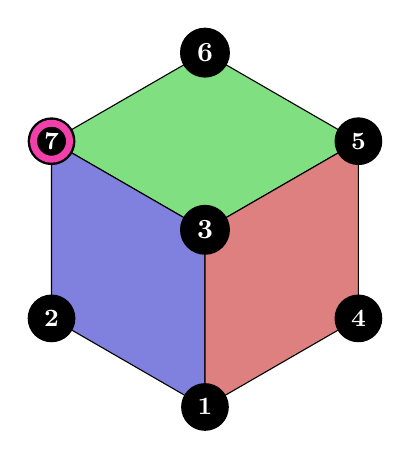
\begin{tikzpicture}
				\coordinate (O) at (0,0);
				\coordinate (A) at ( 30:2.25);
				\coordinate (B) at ( 90:2.25);
				\coordinate (C) at (150:2.25);
				\coordinate (D) at (210:2.25);
				\coordinate (E) at (270:2.25);
				\coordinate (F) at (330:2.25);

				\fill[quantumG, stabilizer] (O) -- (A) -- (B) -- (C) -- cycle;
				\fill[quantumB, stabilizer]  (O) -- (C) -- (D) -- (E) -- cycle;
				\fill[quantumR, stabilizer]  (O) -- (E) -- (F) -- (A) -- cycle;

				\node[data] at (E) {\small $\mathbf{1}$};
				\node[data] at (D) {\small $\mathbf{2}$};
				\node[data] at (O) {$\mathbf{3}$};
				\node[data] at (F) {\small $\mathbf{4}$};
				\node[data] at (A) {\small $\mathbf{5}$};
				\node[data] at (B) {$\mathbf{6}$};
				\node[data] at (C) {\small $\mathbf{7}$};
				\draw[quantumP, line width=2.5pt] (C) circle (6.5pt);
			\end{tikzpicture}
		\end{subfigure}
		\begin{subfigure}[c]{0.62\textwidth}
			\centering
			\begin{quantikz}[row sep=0.6cm]
				\lstick{$\kett{+}$~} & \ctrl{1} &           & \ctrl{3}  &           &
				\slice{} &&&&&& \rstick[7]{~~$\ket{\Op{T}}\sub{L}$} \\
				\lstick{$\kett{0}$~} & \targ{}  & \targ{}   &\phantom{i}& \targ{}   &
				& \ctrl{5}  &&& \ctrl{5}  && \\
				\lstick{$\kett{+}$~} & \ctrl{1} & \ctrl{-1} &\phantom{i}&\phantom{i}& \ctrl{3}
				& \phantom{i}&&&\phantom{i}&& \\
				\lstick{$\kett{0}$~} & \targ{}  & \targ{}   & \targ{}   &\phantom{i}&\phantom{i}
				& \phantom{i}&&&\phantom{i}&& \\
				\lstick{$\kett{+}$~} & \ctrl{1} & \ctrl{-1} &           &\phantom{i}&\phantom{i}
				& \phantom{i}&&&\phantom{i}&& \\
				\lstick{$\kett{0}$~} & \targ{}  & \targ{}   &           &\phantom{i}& \targ{}
				& \phantom{i}&\ctrl{1}&&\phantom{i}& \ctrl{1} & \\[-0.2cm]
				\lstick{$\kett{+}$~} &          & \ctrl{-1} &           & \ctrl{-5} & 
				& \targ{}  & \targ{}  & \gate[style={fill=quantumP}]{\Op{T}^{\dagger}} & \targ{} & \targ{} &
			\end{quantikz}
		\end{subfigure}
		\caption{Modified Steane Code with stabilizer diagram. Note that the abstract circuit can be performed in $8$ steps.}
	\end{figure}

	In the absence of errors, the seven data-qubits are in a logical state $\kett{+}\sub{L}$ once the red line is reached
	
	\begin{equation*}
		\kett{+}\sub{L} \quad=\quad
			\sqrt{\frac{1}{2}}\left(\vphantom{\sqrt{\frac{1}{2}}}
				\kett{0}\sub{L} + \kett{1}\sub{L}
			\right)
		\label{eq:logical-plus-state}
	\end{equation*}

	As pointed out by Austin, the first two \Op{CNOT} gates after the red line result in all the physical states of the logical $\kett{0}\sub{L}$ (resp. $\kett{1}\sub{L}$) having qubit $7$ set to $\kett{0}$ (resp. $\kett{1}$). Once the $e^{i\pi/4}$ phase has been injected by the $\Op{T}^{\dagger}$ gate, the last two \Op{CNOT} gates change the value of qubit $7$ as to return the seven qubits to the state $\kett{+}\sub{L}$. See Figure (\ref{fig:injection-states}) for the detailed superpositions. \\
	
	Note that after the red line, the first two \Op{CNOT} gates bring us out of the Steane Code for the injection and thus collapses the fault distance of our state to $1$; any single error occurring on any of the seven data-qubits corrupts the logical state.

	\subsubsection{Proof of correctness}

	\paragraph{Preparation of $\kett{+}\sub{L}$ } Sticking to our assumed numbering, the stabiliser flows propagate up to the red line as follows

	\begin{equation*}
		\Op{X}_{1} \rightarrow \Op{X}_{124}
		\qquad
		\Op{X}_{3} \rightarrow \Op{X}_{2346}
		\qquad
		\Op{X}_{5} \rightarrow \Op{X}_{456}
		\qquad
		\Op{X}_{7} \rightarrow \Op{X}_{267}
		\qquad
		\Op{Z}_{2} \rightarrow \Op{Z}_{1237}
		\qquad
		\Op{Z}_{4} \rightarrow \Op{Z}_{1345}
		\qquad
		\Op{Z}_{6} \rightarrow \Op{Z}_{3567}
	\end{equation*}

	All those stabilisers commute with one another and we can derive the usual three four-body X-stabilisers
	\begin{equation*}
		\Op{X}_{124}\Op{X}_{2346}\Op{X}_{267} = \Op{X}_{1237}
		\qquad
		\Op{X}_{124}\Op{X}_{2346}\Op{X}_{456} = \Op{X}_{1345}
		\qquad
		\Op{X}_{2346}\Op{X}_{456}\Op{X}_{267} = \Op{X}_{3567}
	\end{equation*}

	The product of the four X-stabiliser flows tells us we have prepared the +1 eigenstate of the observable $\Op{X}\sub{L}$
	\begin{equation*}
		\Op{X}_{1}\Op{X}_{3}\Op{X}_{5}\Op{X}_{7} \rightarrow \Op{X}_{124}\Op{X}_{2346}\Op{X}_{456}\Op{X}_{267} = \Op{X}_{1234567} = \Op{X}\sub{L}
	\end{equation*}

	\paragraph{Injection of $e^{\pi/2}$ phase}

	We need to prove that after the last five steps, assuming we use an $\Op{S}^{\dagger}$ gate instead of the $\Op{T}^{\dagger}$, we find that we have prepared the $+1$ eigenstate of the observable $\Op{Y}\sub{L}$

	\begin{equation*}
		\Op{X}_{1234567}\Op{Z}_{1345} \rightarrow \Op{Y}_{1234567} = \Op{Y}\sub{L}
	\end{equation*}

	\paragraph{(TBD) Injection of $e^{\pi/4}$ phase}

	\newpage

	\subsection{\mbox{\sc Steane Check} --- Detecting code failure}

	This check performs a post-selection based on the syndrome measurement of the $6$ four-body Steane stabilisers in the three plaquettes;
	\begin{equation*}
		\Op{X}_{1237} \qquad\qquad \Op{X}_{1345} \qquad\qquad \Op{X}_{3567}
		\qquad\qquad
		\Op{Z}_{1237} \qquad\qquad \Op{Z}_{1345} \qquad\qquad \Op{Z}_{3567}
	\end{equation*}

	In order to perform this efficiently, a superdense code cycle is used to measure both stabilisers in each plaquettes in parallel. The idling space in the middle is to accommodate the other two plaquettes that need to extract syndromes from the common data qubits.

	\begin{figure}[h!]
		\centering
		\begin{quantikz}[row sep={between origins, 0.75cm}, column sep={between origins, 0.75cm}]
			\lstick{$q\sub{3}$} &&&\targ{}&&&&\ctrl{2}{}&& \\
			\lstick{$q\sub{5}$} &&\targ{}&\phantom{i}&&&\ctrl{1}{}&\phantom{i}&& \\
			\lstick{$\kett{+}$}
			& \ctrl{1} &\ctrl{-1}\gategroup[wires=2, steps=6, style={dashed,rounded corners,fill=quantumG, inner xsep=2pt, inner ysep=-2pt}
            ,background, label style={rounded corners, label position=center, yshift=-0.175cm}]{\sc Bell pair}&\ctrl{-2}&&&\targ{}&\targ{}&\ctrl{1}& \qmeasure{\Op{X}} \\
			\lstick{$\kett{0}$}
			& \targ{} &\ctrl{2}&\ctrl{1}&&&\targ{}&\targ{}&\targ{}& \meter{} \\
			\lstick{$q\sub{6}$} &&\phantom{i}&\targ{}&&&\phantom{i}&\ctrl{-1}&& \\
			\lstick{$q\sub{7}$} &&\targ{}&&&&\ctrl{-2}&&&
		\end{quantikz}
		\caption{Syndrome extraction using superdense coding for stabilisers $\Op{X}_{3567}$ and $\Op{Z}_{3567}$.}
	\end{figure}


	\subsection{\mbox{\sc Phase Check} --- Detecting phase failure}

	This check performs a post-selection based on the syndrome measurement of a single seven-body stabiliser involving all the data qubits.

	{\bf Careful:} $\Op{S}$ is transversal in the Steane Code, $\Op{T}$ is not but $\Op{T}\Op{X}\Op{T}^{\dagger}$ is.
	\begin{figure}[h!]
		\centering
		\begin{quantikz}[row sep={between origins, 0.75cm}]
			\lstick{$q\sub{6}$} & \gate[7,style={rounded corners=5pt}][1cm]{\Op{T}^\dagger}
			& \gate[7,style={rounded corners=5pt}][3cm]{\textsc{Cultivation}}
			& \gate[7,style={rounded corners=5pt}][1cm]{\Op{T}}
			& \\
			\lstick{$q\sub{7}$} &&&& \\
			\lstick{$q\sub{2}$} &&&& \\
			\lstick{$q\sub{3}$} &&&& \\
			\lstick{$q\sub{1}$} &&&& \\
			\lstick{$q\sub{5}$} &&&& \\
			\lstick{$q\sub{4}$} &&&&
		\end{quantikz}
		\caption{Overview of the cultivation stage in three parts.}	
	\end{figure}

	\newpage

	\section{Stage II --- Teleportation}

	The goal of this stage is to move the logical magic state from the Steane Code on $7$ qubits into a Surface Code 

	\newpage

	\appendix

	\section{Preparation stage --- Extra diagrams}

	\begin{figure}[h!]
		\centering
		\scalebox{0.9}{
		\begin{quantikz}[row sep=0.6cm]
			\lstick{$\kett{+}$~} & \ctrl{1} &           & \ctrl{3}  &           &
			\slice{} & \midstick[7]{~~$\begin{aligned}
				  \kett{0000000} &+ \kett{1111111} \\
				+ \kett{1110001} &+ \kett{0001110} \\
				+ \kett{1011100} &+ \kett{0100011} \\ 
				+ \kett{0010111} &+ \kett{1101000} \\ 
				+ \kett{0101101} &+ \kett{1010010} \\
				+ \kett{1100110} &+ \kett{0011001} \\
				+ \kett{1001011} &+ \kett{0110100} \\ 
				+ \kett{0111010} &+ \kett{1000101} \\ 
			\end{aligned}$~~}
			&&& \midstick[7]{~~$\begin{aligned}
				  \kett{0000000} &+ \kett{1111111} \\
				+ \kett{1110000} &+ \kett{0001111} \\
				+ \kett{1011100} &+ \kett{0100011} \\ 
				+ \kett{0010110} &+ \kett{1101001} \\ 
				+ \kett{0101100} &+ \kett{1010011} \\
				+ \kett{1100110} &+ \kett{0011001} \\
				+ \kett{1001010} &+ \kett{0110101} \\ 
				+ \kett{0111010} &+ \kett{1000101} \\ 
			\end{aligned}$~~}
			&&&& \rstick[7]{~~$\ket{\Op{T}}\sub{L}$} \\
			\lstick{$\kett{0}$~} & \targ{}  & \targ{}   &\phantom{i}& \targ{}   &
			&&          & \ctrl{5}  &&& \ctrl{5}  && \\
			\lstick{$\kett{+}$~} & \ctrl{1} & \ctrl{-1} &\phantom{i}&\phantom{i}& \ctrl{3}
			&&          &\phantom{i}&&&\phantom{i}&& \\
			\lstick{$\kett{0}$~} & \targ{}  & \targ{}   & \targ{}   &\phantom{i}&\phantom{i}
			&&          &\phantom{i}&&&\phantom{i}&& \\
			\lstick{$\kett{+}$~} & \ctrl{1} & \ctrl{-1} &           &\phantom{i}&\phantom{i}
			&&          &\phantom{i}&&&\phantom{i}&& \\
			\lstick{$\kett{0}$~} & \targ{}  & \targ{}   &           &\phantom{i}& \targ{}
			&& \ctrl{1} &\phantom{i}&&&\phantom{i}& \ctrl{1} & \\[-0.2cm]
			\lstick{$\kett{+}$~} &          & \ctrl{-1} &           & \ctrl{-5} & 
			&& \targ{}  & \targ{}  && \gate[style={fill=quantumP}]{\Op{T}^{\dagger}} & \targ{} & \targ{} &
		\end{quantikz}
		}
		\caption{Modified Steane Code with intermediate states (normalisation factor omitted). The basis states corresponding to the $\kett{0}\sub{L}$ (resp. $\kett{1}\sub{L}$) are aligned in the left (resp. right) column. Note that the 7-th qubit has a value of $\kett{0}$ (resp. $\kett{1}$) in all the components coming from $\kett{0}\sub{L}$ (resp. $\kett{1}\sub{L}$) before the $\Op{T}^{\dagger}$-gate is applied.}
		\label{fig:injection-states}
	\end{figure}

	\begin{figure}[h!]
		\centering
		\begin{quantikz}[row sep={0.85cm, between origins}, column sep={0.3cm}]
			% Data qubit 6
			\lstick{$q_{6}$} & \gate{\Op{T}^\dagger} && \targ{} &\slice{}&&&&&&&&\slice{}&&\targ{} && \gate{\Op{T}} &
			\\
			% Ancilla 1
			&\wireoverride{n}& \midstick{$\kett{+}$}\wireoverride{n} & \ctrl{-1} && \targ{} &&&
			& &&&\targ{}&&\ctrl{-1} & \qmeasure{\Op{X}} &\swt{n}&
			\\
			% Data qubit 7
			\lstick{$q_{7}$} & \gate{\Op{T}^\dagger} & &\targ{} && \ctrl{-1} &\targ{}&&
			& &&\targ{}&\ctrl{-1}&&\targ{}&&\gate{\Op{T}} &
			\\
			% Ancilla 2
			&\wireoverride{n}& \midstick{$\kett{+}$}\wireoverride{n} & \ctrl{-1} &&&\phantom{i}&&
			& &&\phantom{i}&&&\ctrl{-1}& \qmeasure{\Op{X}} & \swt{n} &
			\\
			% Data qubit 2
			\lstick{$q_{2}$} & \gate{\Op{T}^\dagger} & &\targ{} &&&\phantom{i}&&
			& &&\phantom{i}&&&\targ{}&&\gate{\Op{T}} &
			\\
			% Ancilla 3
			&\wireoverride{n}& \midstick{$\kett{+}$}\wireoverride{n} & \ctrl{-1} &&\targ{}&\phantom{i}&&
			& &&\phantom{i}&\targ{}&&\ctrl{-1}& \qmeasure{\Op{X}} &\swt{n}&
			\\
			% Data qubit 3
			\lstick{$q_{3}$} & \gate{\Op{T}^\dagger} & &\targ{} &&\ctrl{-1}&\ctrl{-4}&\ctrl{3}& \qmeasure{\Op{X}}
			& \wireoverride{}\midstick{$\kett{+}$} &\ctrl{3}&\ctrl{-4}&\ctrl{-1}&&\targ{}&& \gate{\Op{T}} &
			\\
			% Ancilla 4
			&\wireoverride{n}& \midstick{$\kett{+}$}\wireoverride{n} & \ctrl{-1} &&&&\phantom{i}&
			& &\phantom{i}&&&&\ctrl{-1}& \qmeasure{\Op{X}} &\swt{n}&
			\\
			% Data qubit 1
			\lstick{$q_{1}$} & \gate{\Op{T}^\dagger} & &&\targ{}&&&\phantom{i}&
			& &&&&\targ{}&&&\gate{\Op{T}} &
			\\
			% Ancilla 5
			&\wireoverride{n}& \midstick{$\kett{+}$}\wireoverride{n} & \ctrl{1} &\ctrl{-1}&&\ctrl{2}&\targ{}&
			& &\targ{}&\ctrl{2}&&\ctrl{-1}&\ctrl{1}& \qmeasure{\Op{X}} &\swt{n}&
			\\
			% Data qubit 5
			\lstick{$q_{5}$} & \gate{\Op{T}^\dagger} & &\targ{} &&&\phantom{i}&&
			& &&\phantom{i}&&&\targ{}&&\gate{\Op{T}} &
			\\
			% Ancilla 6
			&\wireoverride{n}& \midstick{$\kett{+}$}\wireoverride{n} & \ctrl{1} &&&\targ{}&&
			& &&\targ{}&&&\ctrl{1}& \qmeasure{\Op{X}} &\swt{n}&
			\\
			% Data qubit 4
			\lstick{$q_{4}$} & \gate{\Op{T}^\dagger} & &\targ{} &&&&&
			& &&&&&\targ{}&&\gate{\Op{T}} &
		\end{quantikz}
		\caption{Highlight on the central part of the cultivation in Gidney's circuit. Qubits have been re-ordered for a more readable circuit.}
	\end{figure}

	\newpage

	\section{Teleportation stage --- Qubit layouts}

	\begin{figure}[h!]
		\centering
		\begin{subfigure}[b]{0.95\textwidth}
			\centering
			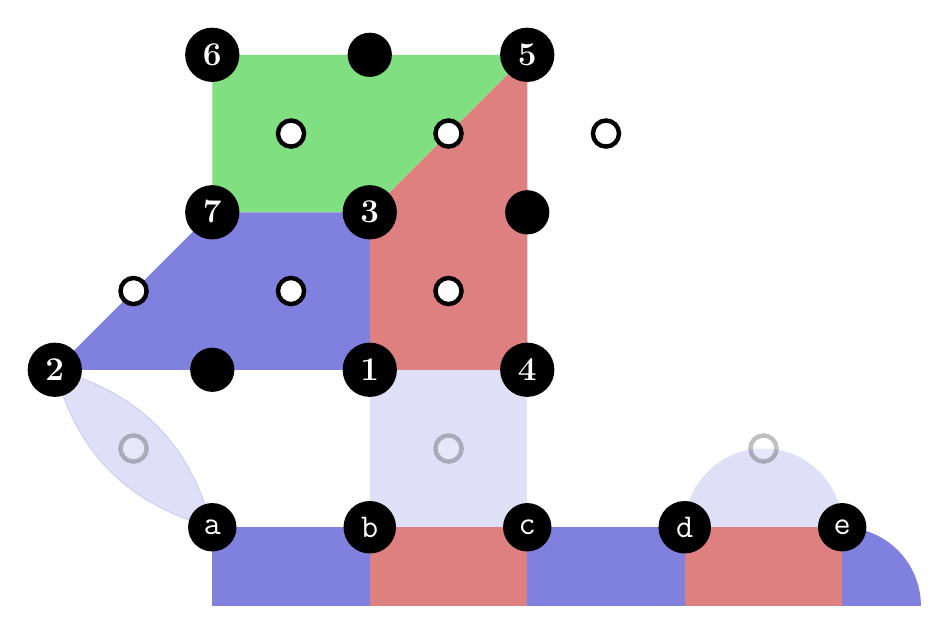
\begin{tikzpicture}
				% Plaquettes of the Steane Code
				\fill[quantumG] (0, 0) -- (4, 0) -- (2,-2) -- (0, -2);
				\fill[quantumB] (0,-2) -- (-2, -4) -- (2, -4) -- (2, -2);
				\fill[quantumR] (2,-2) -- (2, -4) -- (4, -4) -- (4, 0);
	
				% Plaquettes of the Surface Code
				\fill[quantumB] (0,-6) -- (2, -6) -- (2, -7) -- (0, -7);
				\fill[quantumB] (4,-6) -- (6, -6) -- (6, -7) -- (4, -7);
				\fill[quantumR] (2,-6) -- (4, -6) -- (4, -7) -- (2, -7);
				\fill[quantumR] (6,-6) -- (8, -6) -- (8, -7) -- (6, -7);
	
				\fill[quantumB, opacity=0.25] (6, -6) arc[start angle=180, end angle=0, radius=1.0]
					-- (8, -6) -- cycle;
				\fill[quantumB] (8, -6) arc[start angle=90, end angle=0, radius=1.0]
					-- (8, -7) -- cycle;
	
				\fill[quantumB, opacity=0.25] (2,-4) -- (4, -4) -- (4, -6) -- (2, -6);
				\filldraw[quantumB, opacity=0.25] (-2,-4) to[bend left=30] (0,-6) to[bend left=30] (-2,-4);
		
				\node[data] at (2, 0) {\phantom{o}};
				\node[data] at (4,-2) {\phantom{o}};
				\node[data] at (0,-4) {\phantom{o}};
	
				\node[data] at (2,-4) {\large $\mathbf{1}$};
				\node[data] at (-2,-4) {\large $\mathbf{2}$};
				\node[data] at (2,-2) {\large $\mathbf{3}$};
				\node[data] at (4,-4) {\large $\mathbf{4}$};
				\node[data] at (4, 0) {\large $\mathbf{5}$};
				\node[data] at (0, 0) {\large $\mathbf{6}$};
				\node[data] at (0,-2) {\large $\mathbf{7}$};	
	
				\foreach \x in {1, 3, 5}{ \node[meas] at (\x,-1) {}; }
				\foreach \x in {-1, 1, 3}{ \node[meas] at (\x,-3) {}; }
				\foreach \x in {-1, 3, 7}{ \node[meas, opacity=0.25] at (\x,-5) {}; }
	
%				\foreach \x in {0, 2, 4, 6, 8}{ \node[data] at (\x, -6) {\phantom{o}}; }
				\node[data] at (0, -6) {\large\tt a};
				\node[data] at (2, -6) {\large\tt b};
				\node[data] at (4, -6) {\large\tt c};
				\node[data] at (6, -6) {\large\tt d};
				\node[data] at (8, -6) {\large\tt e};
			\end{tikzpicture}
			\caption{Modified Steane Code overlaid on the surface code array. Data qubits are identified as black circles. Measurement qubits are shown as white circles. The extra qubits (6 syndrome and 3 data) can be used to perform the superdense code cycle and the cultivation stage. The surface code onto which the magic state will be teleported is partially shown below for reference.}
		\end{subfigure}
		\vspace{0.5cm}
		\begin{subfigure}[b]{0.45\textwidth}
			\centering
			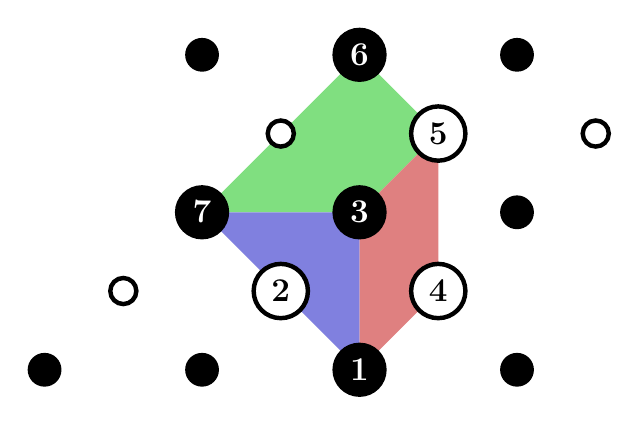
\begin{tikzpicture}
				% Plaquettes of the Steane Code
				\fill[quantumG] (2, 0) -- (3,-1) -- (2,-2) -- (0, -2);
				\fill[quantumB] (0,-2) -- (2, -4) -- (2, -2);
				\fill[quantumR] (2,-2) -- (3, -1) -- (3, -3) -- (2,-4);

				\node[data] at ( 2, 0) {\phantom{.}};
				\node[data] at ( 4,-2) {\phantom{.}};
				\node[data] at ( 0,-4) {\phantom{.}};
				\node[data] at (-2,-4) {\phantom{.}};

				\node[data] at (2,-4) {\large $\mathbf{1}$};
				\node[meas] at (1,-3) {\large $\mathbf{2}$};
				\node[data] at (2,-2) {\large $\mathbf{3}$};
				\node[meas] at (3,-3) {\large $\mathbf{4}$};
				\node[meas] at (3,-1) {\large $\mathbf{5}$};
				\node[data] at (2, 0) {\large $\mathbf{6}$};
				\node[data] at (0,-2) {\large $\mathbf{7}$};	

				\node[data] at ( 0, 0) {\phantom{.}};
				\node[data] at ( 4, 0) {\phantom{.}};
				\node[data] at ( 4,-4) {\phantom{.}};

				\foreach \x in {1, 5}{ \node[meas] at (\x,-1) {}; }
				\node[meas] at (-1,-3) {};
			\end{tikzpicture}
			\caption{Initial locations of the $7$ qubits for the Steane Code}
		\end{subfigure}
		\begin{subfigure}[b]{0.45\textwidth}
			\centering
			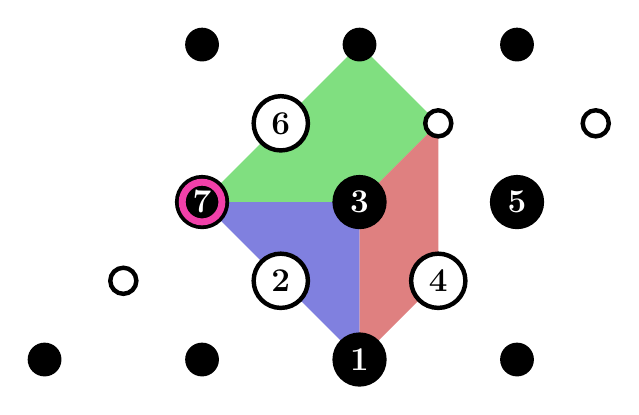
\begin{tikzpicture}
				% Plaquettes of the Steane Code
				\fill[quantumG] (2, 0) -- (3,-1) -- (2,-2) -- (0, -2);
				\fill[quantumB] (0,-2) -- (2, -4) -- (2, -2);
				\fill[quantumR] (2,-2) -- (3, -1) -- (3, -3) -- (2,-4);

				\node[data] at ( 2, 0) {\phantom{.}};
				\node[data] at ( 4,-2) {\phantom{.}};
				\node[data] at ( 0,-4) {\phantom{.}};
				\node[data] at (-2,-4) {\phantom{.}};

				\node[data] at (2,-4) {\large $\mathbf{1}$};
				\node[meas] at (1,-3) {\large $\mathbf{2}$};
				\node[data] at (2,-2) {\large $\mathbf{3}$};
				\node[meas] at (3,-3) {\large $\mathbf{4}$};
				\node[data] at (4,-2) {\large $\mathbf{5}$};
				\node[meas] at (1,-1) {\large $\mathbf{6}$};
				\node[data] at (0,-2) {\large $\mathbf{7}$};	
				\node[circle, draw=quantumP, line width=2.5pt] at (0,-2) {\scalebox{0.75}{\phantom{o}}};

				\node[data] at ( 0, 0) {\phantom{.}};
				\node[data] at ( 4, 0) {\phantom{.}};
				\node[data] at ( 4,-4) {\phantom{.}};

				\foreach \x in {3, 5}{ \node[meas] at (\x,-1) {}; }
				\node[meas] at (-1,-3) {};
			\end{tikzpicture}
			\caption{Locations of the $7$ qubits when the $\Op{T}^\dagger$ gate is applied}
		\end{subfigure}
	\end{figure}

	\begin{figure}[h!]
		\centering
		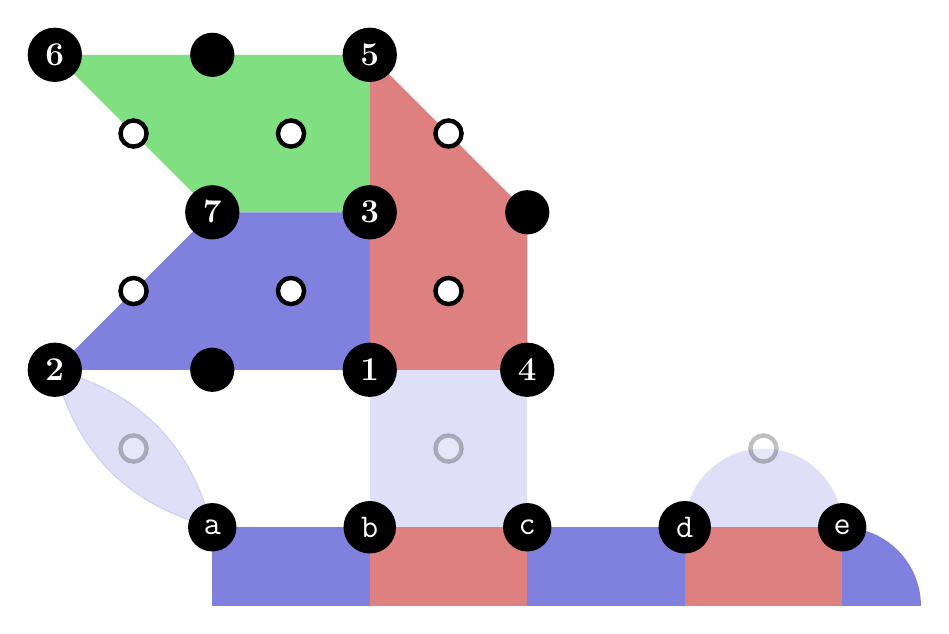
\begin{tikzpicture}
			% Plaquettes of the Steane Code
			\fill[quantumG] (-2, 0) -- ( 2, 0) -- ( 2,-2) -- ( 0,-2);
			\fill[quantumB]  ( 0,-2) -- (-2,-4) -- ( 2,-4) -- ( 2,-2);
			\fill[quantumR]   ( 2, 0) -- ( 4,-2) -- ( 4,-4) -- ( 2,-4);

			% Plaquettes of the Surface Code
			\fill[quantumB] (0,-6) -- (2, -6) -- (2, -7) -- (0, -7);
			\fill[quantumB] (4,-6) -- (6, -6) -- (6, -7) -- (4, -7);
			\fill[quantumR] (2,-6) -- (4, -6) -- (4, -7) -- (2, -7);
			\fill[quantumR] (6,-6) -- (8, -6) -- (8, -7) -- (6, -7);

			\fill[quantumB, opacity=0.25] (6, -6) arc[start angle=180, end angle=0, radius=1.0]
				-- (8, -6) -- cycle;
			\fill[quantumB] (8, -6) arc[start angle=90, end angle=0, radius=1.0]
				-- (8, -7) -- cycle;

			\fill[quantumB, opacity=0.25] (2,-4) -- (4, -4) -- (4, -6) -- (2, -6);
			\filldraw[quantumB, opacity=0.25] (-2,-4) to[bend left=30] (0,-6) to[bend left=30] (-2,-4);


			\node[data] at ( 0, 0) {\phantom{o}};
			\node[data] at ( 4,-2) {\phantom{o}};
			\node[data] at ( 0,-4) {\phantom{o}};

			\node[data] at ( 2,-4) {\large $\mathbf{1}$};
			\node[data] at (-2,-4) {\large $\mathbf{2}$};
			\node[data] at ( 2,-2) {\large $\mathbf{3}$};
			\node[data] at ( 4,-4) {\large $\mathbf{4}$};
			\node[data] at ( 2, 0) {\large $\mathbf{5}$};
			\node[data] at (-2, 0) {\large $\mathbf{6}$};
			\node[data] at ( 0,-2) {\large $\mathbf{7}$};	

			\foreach \x in {-1, 1, 3}{
				\foreach \y in {-3, -1}{
					\node[meas] at (\x,\y) {};
				}
			}
			\foreach \x in {-1, 3, 7}{ \node[meas, opacity=0.25] at (\x,-5) {}; }

			\node[data] at (0, -6) {\large\tt a};
			\node[data] at (2, -6) {\large\tt b};
			\node[data] at (4, -6) {\large\tt c};
			\node[data] at (6, -6) {\large\tt d};
			\node[data] at (8, -6) {\large\tt e};
		\end{tikzpicture}
		\caption{(Alternative) Modified Steane Code overlaid on the surface code array. Data qubits are identified as black circles. Measurement qubits are shown as white circles. The extra qubits (6 syndrome and 3 data) can be used to perform the superdense code cycle and the cultivation stage. The surface code onto which the magic state will be teleported is partially shown below for reference.}
	\end{figure}

	\newpage

	\section{Teleportation stage --- Observable tracking}

	There are two observables that are going to be moved into the target Surface Code in the teleportation stage; $\Op{X}\sub{267}$ and $\Op{Z}\sub{124}$.

	\begin{figure}[h!]
		\centering
		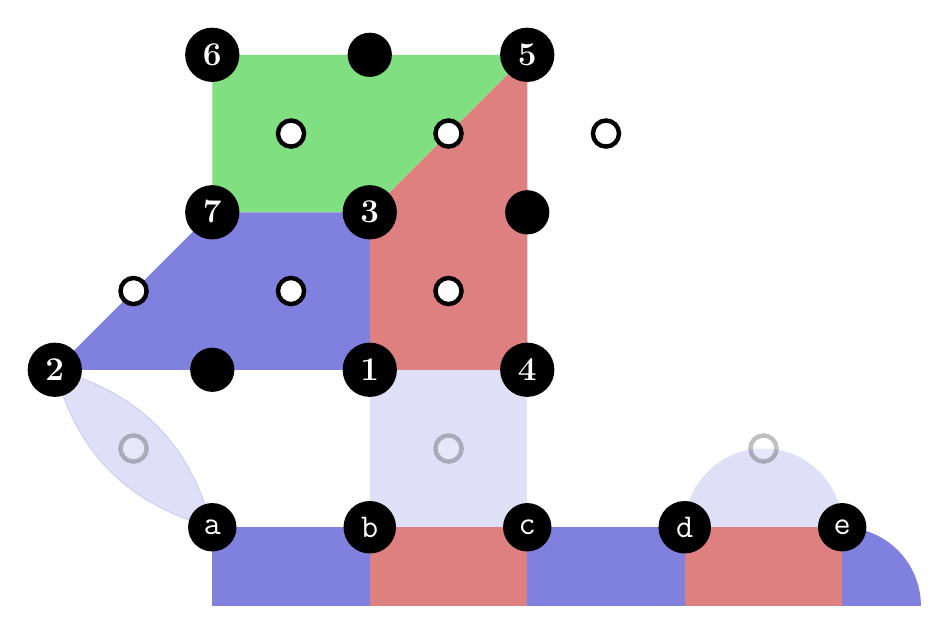
\begin{tikzpicture}
			% Plaquettes of the Steane Code
			\fill[quantumG] (0, 0) -- (4, 0) -- (2,-2) -- (0, -2);
			\fill[quantumB] (0,-2) -- (-2, -4) -- (2, -4) -- (2, -2);
			\fill[quantumR] (2,-2) -- (2, -4) -- (4, -4) -- (4, 0);

			% Plaquettes of the Surface Code
			\fill[quantumB] (0,-6) -- (2, -6) -- (2, -7) -- (0, -7);
			\fill[quantumB] (4,-6) -- (6, -6) -- (6, -7) -- (4, -7);
			\fill[quantumR] (2,-6) -- (4, -6) -- (4, -7) -- (2, -7);
			\fill[quantumR] (6,-6) -- (8, -6) -- (8, -7) -- (6, -7);

			\fill[quantumB, opacity=0.25] (6, -6) arc[start angle=180, end angle=0, radius=1.0]
				-- (8, -6) -- cycle;
			\fill[quantumB] (8, -6) arc[start angle=90, end angle=0, radius=1.0]
				-- (8, -7) -- cycle;

			\fill[quantumB, opacity=0.25] (2,-4) -- (4, -4) -- (4, -6) -- (2, -6);
			\filldraw[quantumB, opacity=0.25] (-2,-4) to[bend left=30] (0,-6) to[bend left=30] (-2,-4);
	
			\node[data] at (2, 0) {\phantom{o}};
			\node[data] at (4,-2) {\phantom{o}};
			\node[data] at (0,-4) {\phantom{o}};

			\node[data] at (2,-4) {\large $\mathbf{1}$};
			\node[data] at (-2,-4) {\large $\mathbf{2}$};
			\node[data] at (2,-2) {\large $\mathbf{3}$};
			\node[data] at (4,-4) {\large $\mathbf{4}$};
			\node[data] at (4, 0) {\large $\mathbf{5}$};
			\node[data] at (0, 0) {\large $\mathbf{6}$};
			\node[data] at (0,-2) {\large $\mathbf{7}$};	

			\foreach \x in {1, 3, 5}{ \node[meas] at (\x,-1) {}; }
			\foreach \x in {-1, 1, 3}{ \node[meas] at (\x,-3) {}; }
			\foreach \x in {-1, 3, 7}{ \node[meas, opacity=0.25] at (\x,-5) {}; }

			\node[data] at (0, -6) {\large\tt a};
			\node[data] at (2, -6) {\large\tt b};
			\node[data] at (4, -6) {\large\tt c};
			\node[data] at (6, -6) {\large\tt d};
			\node[data] at (8, -6) {\large\tt e};
		\end{tikzpicture}
		\caption{Qubit layout \#1 considered for the teleportation}
	\end{figure}

	The lattice surgery is performed in three rounds with different types of syndrome measurements.

	\textbf{Superdense} means that it uses a GHZ state to measure both X/Z-stabilizers in parallel in each plaquette.
	
	\textbf{Extended} means that it uses a GHZ state but only Z-stabilizers are measured.
	
	\textbf{Syndrome} means the usual syndrome measurement of the surface code.
	
	\textbf{Destructive} means that the data qubits are directly measured and the syndromes are computed by XOR'ing the corresponding classical measurements results

	\begin{figure}[h!]
		\centering
		\begin{tabular}{|c|c|c|c|c|}
			\hline
			Operator & Round 1 & Round 2 & Round 3 & Purpose \\\hline\hline
			$\Op{X}\sub{1237}$ & n/a & n/a & Destructive & Post-selection of $\Op{X}\sub{1237ab}$ \\
			$\Op{Z}\sub{1237}$ & Extended & Extended & n/a & Post-selection \\
			$\Op{X}\sub{1345}$ & Superdense & n/a & Destructive & Post-selection \\
			$\Op{Z}\sub{1345}$ & Superdense & Extended & n/a & Post-selection \\
			$\Op{X}\sub{3567}$ & Superdense & n/a & Destructive & Post-selection \\
			$\Op{Z}\sub{3567}$ & Superdense & Extended & n/a & Post-selection \\
			$\Op{X}_{ab}$ & n/a & n/a & Syndrome & Post-selection of $\Op{X}\sub{1237ab}$ \\
			\hline
		\end{tabular}
		\caption{Summary of measurements involved in the Steane Code}
	\end{figure}

	In order to turn the logical operator $\Op{Z}\sub{124}$ into $\Op{Z}_{\mbox{\scriptsize\tt abcde}}$, we measure the following stabilizers and the parity of their three measurement results gives us the sign relationship between these two logical operators

	\begin{equation*}
		p\sub{\Op{Z}} ~=~ (-1)^{\bar{\Op{Z}}_{2\tt a}}(-1)^{\bar{\Op{Z}}_{14\tt bc}}(-1)^{\bar{\Op{Z}}_{\tt de}}
	\end{equation*}

	In order to turn the logical operator $\Op{X}\sub{267}$ into $\Op{X}_{\scriptstyle\tt afghi}$ ({\tt fghi} are the data qubits vertically aligned below {\tt a}), we simply use the parity of the three results of the destructive measurements on qubits $2$, $6$ and $7$ to determine the sign relationship between these two logical operators.

	\newpage
	
	\section{\Op{T}-gate construct}

	We will use the following identities throughout this section. Normalisation constants are dropped for convenience.
	\begin{equation*}
		\sigma = e\Sup{i\frac{\pi}{2}}
		\qquad\qquad
		\ket{\Op{S}} = \kett{0} + \sigma\kett{1}
		\qquad\qquad
		\tau = e\Sup{i\frac{\pi}{4}}		
		\qquad\qquad
		\ket{\Op{T}} = \kett{0} + \tau\kett{1}
		\qquad\qquad
		\sigma\Sup{2} = -1
		\qquad\qquad
		\tau\Sup{2} = \sigma
	\end{equation*}

	While we can apply a \Op{T}-gate on a single physical qubit directly, applying it transversally on a surface code does not perform a logical \Op{T}-gate. Instead, we use the following construct on the surface code to realise a \Op{T}-gate\footnote{All the states and gates involved can be thought as either physical for a single qubit or logical for a surface code.}.
	\begin{figure}[h!]
		\centering
		\begin{quantikz}[column sep=0.5cm]
			\lstick{$\ket{\psi}$}
				& \targ{}
				& \meter{}
				& \ctrl[vertical wire=c]{2}\wire[l][1]["\tt m"{above, pos=0.65}]{c}\swt{c}
				& 
				& 
				& \ctrl[vertical wire=c]{1}
				& \swt{n}
				& 
			\\
			\lstick{$\ket{\Op{S}}$}
				& \phantom{n}
				& 
				& \phantom{n}
				&
				& \targ{}\gategroup[wires=2, steps=3, style={dashed,rounded corners,fill=blue!20, xshift=-1pt, inner xsep=3pt, inner ysep=2pt}
            ,background, label style={rounded corners, label position=below, yshift=-0.5cm}]{\Op{S}-correction}
				& \qmeasure{\Op{X} or \Op{Z}}
				& \ctrl[vertical wire=c]{1}\wire[l][1]["\tt s"{above, pos=0.65}]{c}\swt{c}
				& \swt{n}
			\\
			\lstick{$\ket{\Op{T}}$}
				& \ctrl{-2}
				& 
				& \gate{\Op{X}}
				& 
				& \ctrl{-1}
				& 
				& \gate{\Op{Z}}
				& 
			\rstick{$\Op{T}\ket{\psi}$}
		\end{quantikz}
		\caption{Abstract circuit for performing a \Op{T}-gate on an arbitrary state.}
	\end{figure}

%	\begin{figure}[h!]
%		\centering
%		\begin{subfigure}[b]{0.325\textwidth}
%			\centering
%			\begin{quantikz}
%				\lstick{$\ket{\psi}$}
%				& \targ{} & \meter{} & \ctrl[vertical wire=c]{1}\swt{c} & \ctrl[vertical wire=c]{1} & \swt{n} \\
%				\lstick{$\ket{\Op{S}}$}
%				& \ctrl{-1} &          &       \gate{\Op{X}}     & \gate{\Op{Z}} &
%				\rstick{$\Op{S}\ket{\psi}$}
%			\end{quantikz}
%			\caption{Gadget for applying an \Op{S}-gate.}
%		\end{subfigure}
%		\begin{subfigure}[b]{0.45\textwidth}
%			\centering
%			\begin{quantikz}
%				\lstick{$\ket{\psi}$}
%				& \targ{} & \meter{} & \ctrl[vertical wire=c]{1}\swt{c} & \ctrl[vertical wire=c]{1} & \swt{n} \\
%				\lstick{$\ket{\Op{T}}$}
%				& \ctrl{-1} &          &       \gate{\Op{X}}     & \gate{\Op{S}} &
%				\rstick{$\Op{T}\ket{\psi}$}
%			\end{quantikz}
%			\caption{Gadget for applying a \Op{T}-state.}
%		\end{subfigure}
%		\begin{subfigure}[b]{0.45\textwidth}
%			\centering
%			\begin{quantikz}
%				\lstick{$\ket{\psi}$}
%				& \ctrl{1} &          & \gate{\Op{Z}} & \\
%				\lstick{$\ket{\Op{S}}$}
%				& \targ{ } & \qmeasure{\Op{X} or \Op{Z}} & \ctrl[vertical wire=c]{-1}\swt{c} & \swt{n}
%			\end{quantikz}
%			\caption{Gadget for a classically-controlled \Op{S}-correction.}
%		\end{subfigure}
%		\caption{Abstract circuits for performing a \Op{T}-gate on an arbitrary state.}
%	\end{figure}

	\subsection{Proof of correctness : \Op{S}-correction}

	We will prove that the blue sub-circuit performs a conditional \Op{S}-gate on an arbitrary quantum state based on the input bit {\tt m}.
	\begin{align*}
		\parentheses{\kett{0} + \sigma\kett{1}}
		\parentheses{\alpha\sub{0}\kett{0} + \alpha\sub{1}\kett{1}}
		~=&~~
			\alpha\sub{0}\kett{00} + \alpha\sub{1}\kett{01} + \sigma\alpha\sub{0}\kett{10} + \sigma\alpha\sub{1}\kett{11}
		\\
		~\rightarrow&~~
			\alpha\sub{0}\kett{00} + \alpha\sub{1}\kett{11} + \sigma\alpha\sub{0}\kett{10} + \sigma\alpha\sub{1}\kett{01}
		\tag{\Op{CNOT}}
		\\
		~=&~~
			\kett{0}\parentheses{\alpha\sub{0}\kett{0} + \sigma\alpha\sub{1}\kett{1}}
			+ \kett{1}\parentheses{\sigma\alpha\sub{0}\kett{0} + \alpha\sub{1}\kett{1}}
	\end{align*}

	Based on the value of the input bit {\tt m}, we will perform the measurement either in the \Op{X}-basis or the \Op{Z}-basis.

	\paragraph{Case {\tt m = 0}.} We apply an \Op{H} gate on the left qubit prior to measurement.
	\begin{align*}
		\kett{+}\parentheses{\alpha\sub{0}\kett{0} + \sigma\alpha\sub{1}\kett{1}}
			+ \kett{-}\parentheses{\sigma\alpha\sub{0}\kett{0} + \alpha\sub{1}\kett{1}}
%		~=&~~
%			\sqrt{\frac{1}{2}}\brackets{
%				\alpha\sub{0}\kett{00} + \sigma\alpha\sub{1}\kett{01} + \alpha\sub{0}\kett{10} + \sigma\alpha\sub{1}\kett{11}
%				+ \sigma\alpha\sub{0}\kett{00} + \alpha\sub{1}\kett{01} - \sigma\alpha\sub{0}\kett{10} - \alpha\sub{1}\kett{11}
%			}
%		\\
		~~=&~~
			\frac{1+\sigma}{\sqrt{2}}\kett{0}\parentheses{\alpha\sub{0}\kett{0} + \alpha\sub{1}\kett{1}}
			+
			\frac{1-\sigma}{\sqrt{2}}\kett{1}\parentheses{\alpha\sub{0}\kett{0} - \alpha\sub{1}\kett{1}}
	\end{align*}
	If we measure the left qubit as {\tt s = 0}, then the state on the right qubit is already correct. On the other hand, if we measure the left qubit as {\tt s = 1}, then the state on the right qubit will undergo a \Op{Z}-correction.

	\paragraph{Case {\tt m = 1}.} If we measure the left qubit as {\tt s = 0}, then the state on the right qubit is already correct. On the other hand, if we measure the left qubit as {\tt s = 1}, then the state on the right qubit will undergo a \Op{Z}-correction.
	\begin{equation*}
		\sigma\alpha\sub{0}\kett{0} + \alpha\sub{1}\kett{1}
		~~\xrightarrow{\Op{Z}}~~ \sigma\alpha\sub{0}\kett{0} - \alpha\sub{1}\kett{1}
		~~=~~ \sigma\alpha\sub{0}\kett{0} + \sigma\Sup{2}\alpha\sub{1}\kett{1}
		~~=~~ \sigma\parentheses{\alpha\sub{0}\kett{0} + \sigma\alpha\sub{1}\kett{1}}
	\end{equation*}
	and we are left with a state which is equal (up to a global phase of $\sigma$) to the desired output of an \Op{S}-gate.

	\subsection{Proof of correctness : \Op{T}-construct}

	We can prove that the complete circuit performs a \Op{T}-gate on an arbitrary quantum state.
	\begin{align*}
		\parentheses{\alpha\sub{0}\kett{0} + \alpha\sub{1}\kett{1}}\parentheses{\kett{0}+\tau\kett{1}}
		~=&~~ \alpha\sub{0}\kett{00} + \alpha\sub{0}\tau\kett{01} + \alpha\sub{1}\kett{10} + \alpha\sub{1}\tau\kett{11} \\
		~\rightarrow&~~
			\alpha\sub{0}\kett{00} + \alpha\sub{0}\tau\kett{11} + \alpha\sub{1}\kett{10} + \alpha\sub{1}\tau\kett{01}
		\tag{\Op{CNOT}} \\[2pt]
		~=&~ \kett{0}\parentheses{\alpha\sub{0}\kett{0} + \alpha\sub{1}\tau\kett{1}} + 
			\kett{1}\parentheses{\alpha\sub{0}\tau\kett{1} + \alpha\sub{1}\kett{0}}
	\end{align*}

	If we measure the top qubit as {\tt m = 0}, then the state on the bottom qubit is already the desired output of the \Op{T}-gate construct. On the other hand, if we measure the top qubit as {\tt m = 1}, then the state on the bottom qubit will undergo both corrections\footnote{Since the \Op{X}-correction is a Pauli correction, it is sufficient to include the bit {\tt m} in the tracking of any \Op{Z}-observable passing through it.}
	\begin{equation*}
		\alpha\sub{0}\tau\kett{1} + \alpha\sub{1}\kett{0}
		~~\xrightarrow{\Op{X}}~~ \alpha\sub{0}\tau\kett{0} + \alpha\sub{1}\kett{1}
		~~\xrightarrow{\Op{S}}~~ \alpha\sub{0}\tau\kett{0} + \sigma\alpha\sub{1}\kett{1}
		~~=~~ \alpha\sub{0}\tau\kett{0} + \alpha\sub{1}\tau\Sup{2}\kett{1}
		~~=~~ \tau\parentheses{\alpha\sub{0}\kett{0} + \alpha\sub{1}\tau\kett{1}}
	\end{equation*}
	and we are left with a state which is equal (up to a global phase of $\tau$) to the desired output of a \Op{T}-gate.

	\newpage

	\begin{figure}
		\centering
		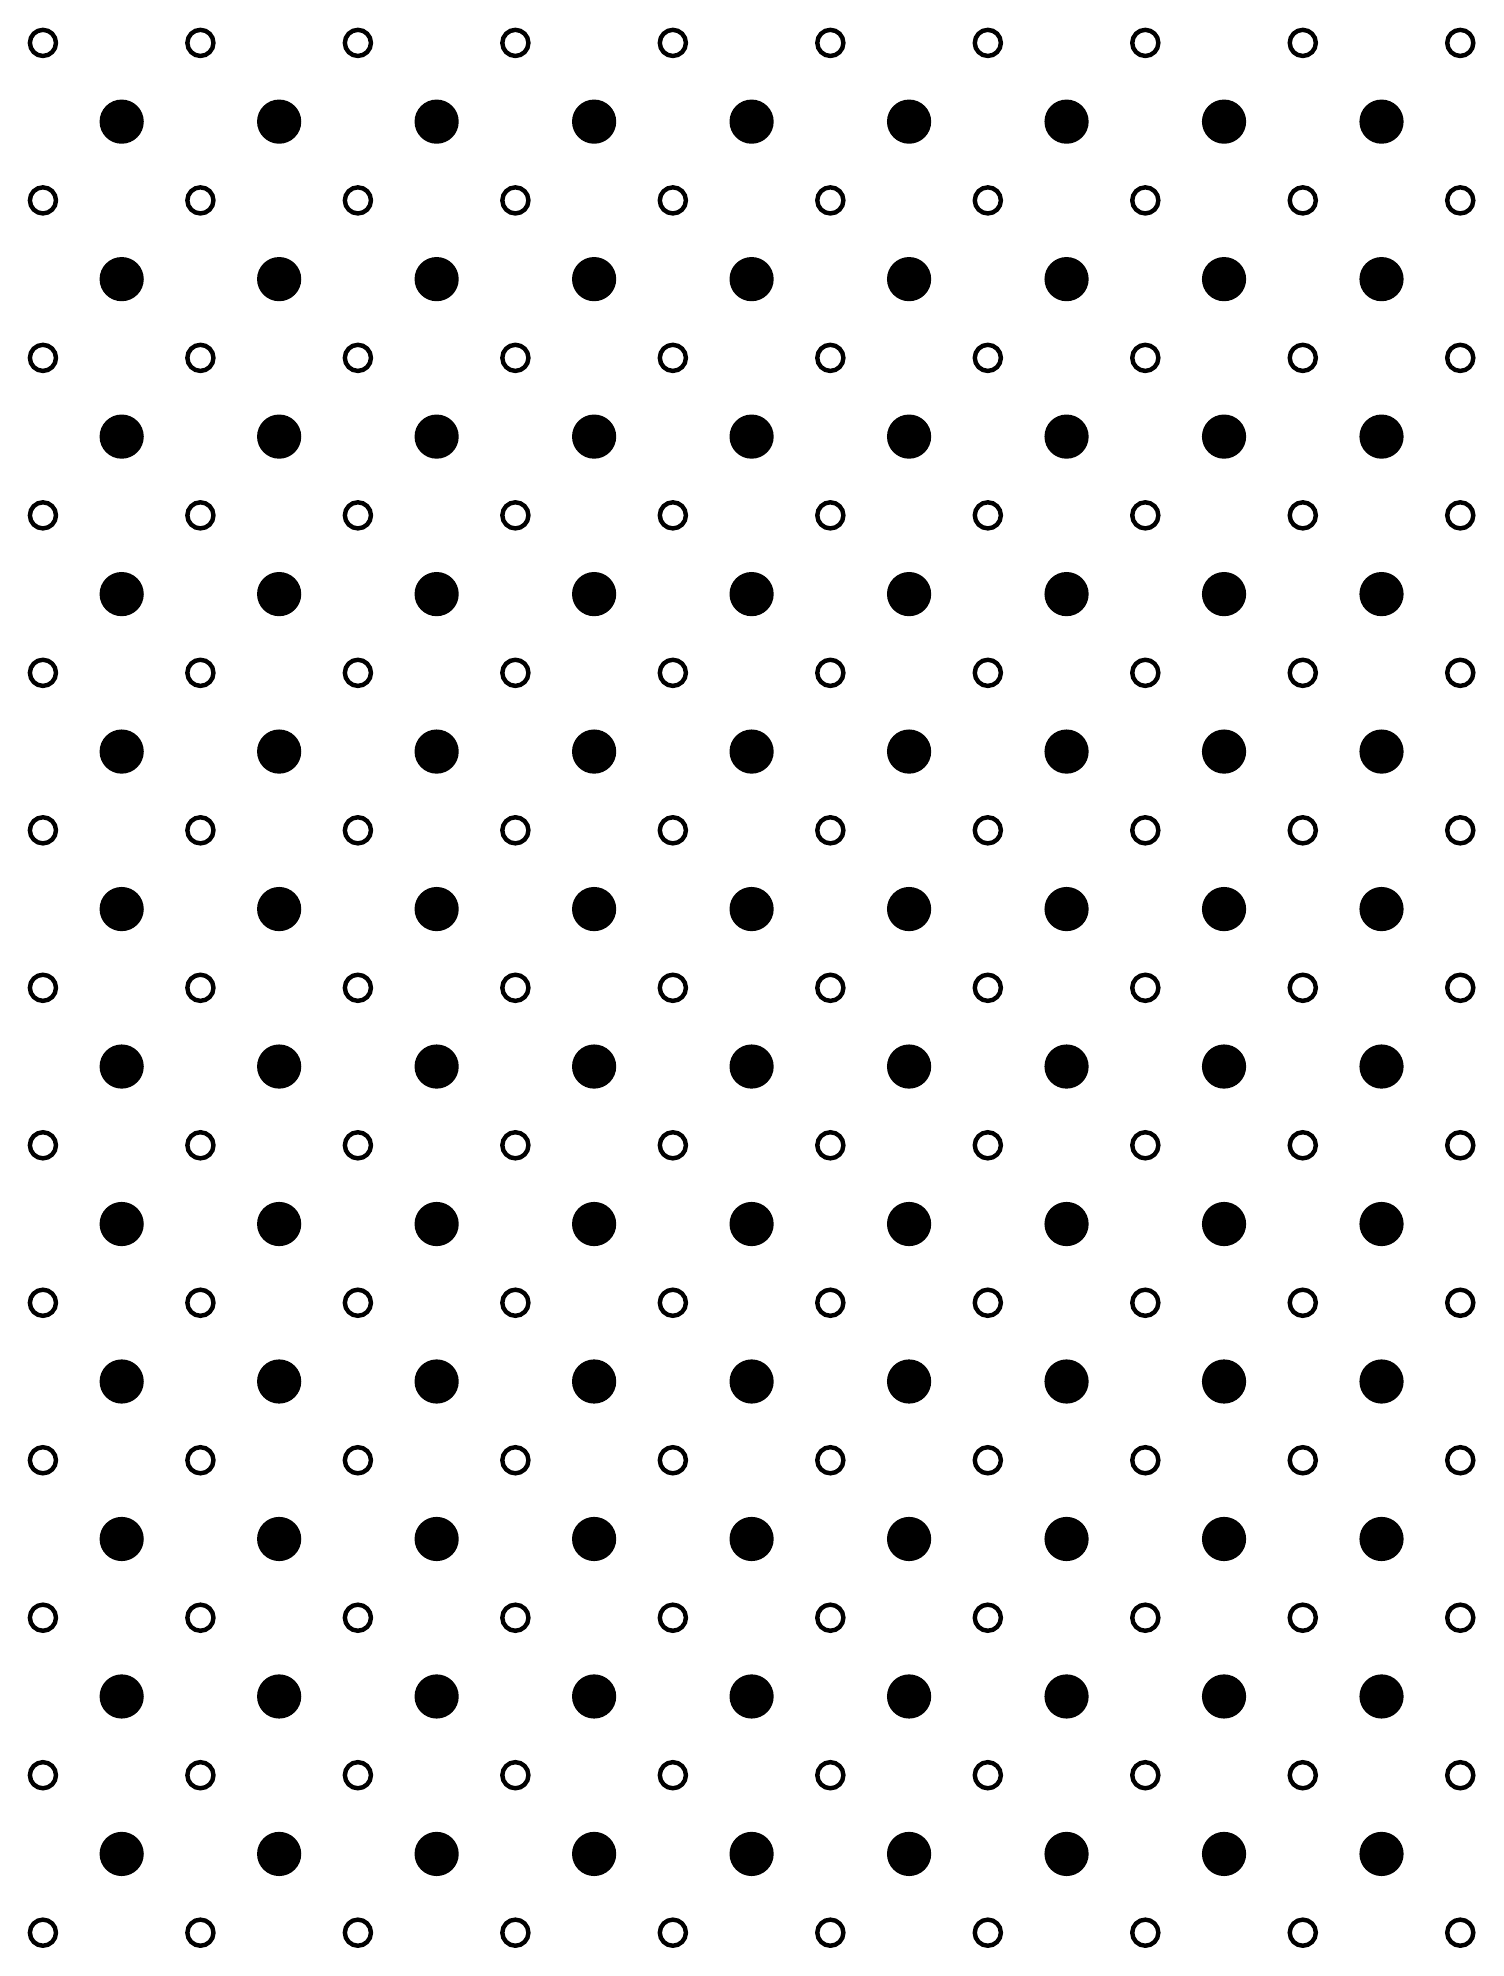
\begin{tikzpicture}
			\foreach \x in {2, 4, 6, 8, 10, 12, 14, 16, 18}{
				\foreach \y in {2, 4, 6, 8, 10, 12, 14, 16, 18, 20, 22, 24}{
					\node[data] at (\x,\y) {\phantom{o}};
				}
			}
			\foreach \x in {1, 3, 5, 7, 9, 11, 13, 15, 17, 19}{
				\foreach \y in {1, 3, 5, 7, 9, 11, 13, 15, 17, 19, 21, 23, 25}{
					\node[meas] at (\x,\y) {};
				}
			}
		\end{tikzpicture}
	\end{figure}

\end{document}
